\chapter{\label{ch:ch01}ГЛАВА 1} % Нужно сделать главу в содержании заглавными буквами

\section{\label{sec:ch01/sec01}Раздел 1: Теоретические основы}
\subsection{\label{subsec:ch01/sec01/sub01}Описание языка Python}

Python - это высокоуровневый интерпретируемый язык программирования, который отличается простотой и понятностью синтаксиса. Он поддерживает различные парадигмы программирования, включая процедурное, объектно-ориентированное и функциональное программирование.

Python используется для разработки веб-приложений, научных вычислений, анализа данных, искусственного интеллекта, машинного обучения и других областей. Он имеет обширную стандартную библиотеку, которая включает в себя модули для работы с различными типами данных, сетевыми протоколами, графикой и д.р.

Python поддерживает динамическую типизацию и автоматическое управление памятью, что упрощает процесс разработки и делает его более гибким. Кроме того, Python является кроссплатформенным языком, что означает, что программы, написанные на нем, могут быть запущены на различных операционных системах без изменений.

В этом курсовом проекте Python будет использовано в связке с его модулем PyQT для создание игры "2048"

\subsection{\label{subsec:ch01/sec01/sub01}Описание библиотеки PyQT}
PyQT - это набор библиотек для разработки графических пользовательских интерфейсов (GUI) на языке программирования Python. Она предоставляет доступ к функциональности библиотеки Qt, которая является одной из самых популярных и мощных библиотек для создания GUI.

Основные особенности PyQT:
\begin{enumerate}
\item Кроссплатформенность: PyQT поддерживает работу на различных операционных системах, таких как Windows, macOS и Linux.
\item Обширный набор виджетов: PyQT предоставляет широкий выбор готовых виджетов для создания интерфейсов, таких как кнопки, текстовые поля, таблицы и многое другое.
\item Графический дизайн: с помощью PyQT можно легко создавать стильные и современные пользовательские интерфейсы с использованием каскадных таблиц стилей (CSS).
\item  Событийная модель: PyQT обладает мощной системой обработки событий, что позволяет реагировать на действия пользователя, такие как нажатия клавиш, перемещения мыши и т.д.
\end{enumerate}

\subsection{\label{subsec:ch01/sec01/sub01} }

\chapter{\label{ch:ch02}ГЛАВА 2} 

\section{\label{sec:ch01/sec01}Раздел 1: Практика}

\subsection{\label{subsec:ch01/sec01/sub01}Описание игры "2048"}

Игра 2048 - это логическая головоломка, в которой игроку нужно объединять одинаковые числа, чтобы получить число 2048 или достичь максимального возможного числа на игровом поле На поле определенного размера.

Описание алгоритма игры 2048:
\begin{itemize}
\item Начало игры:

   - На игровом поле появляются две плитки со случайными значениями 2 или 4.
   - Игрок может управлять плитками с помощью стрелок на клавиатуре (вверх, вниз, влево, вправо).
\item Ход игрока:

   - При каждом ходе все плитки на игровом поле сдвигаются в выбранном направлении (вверх, вниз, влево, вправо).
   - Если две плитки с одинаковыми значениями сталкиваются при сдвиге, они объединяются в одну плитку с удвоенным значением.
   - После каждого хода на свободной клетке появляется новая плитка со значением 2 или 4.
\item  Цель игры:

   - Цель игры 2048 заключается в том, чтобы получить плитку со значением 2048 путем объединения плиток с одинаковыми значениями.
   - Если на игровом поле больше нет свободных клеток или невозможно выполнить ход, игра завершается.
\item Победа и поражение:

   - Игрок выигрывает, если он достигает плитки со значением 2048.
   - Игрок проигрывает, если на игровом поле больше нет свободных клеток и он не может выполнить дальнейшие ходы.
\item Стратегия:

   - Для успешного прохождения игры рекомендуется стратегия объединения плиток с наименьшими значениями, чтобы освободить место для новых плиток и предотвратить блокировку поля.
\end{itemize}
\subsection{\label{subsec:ch01/sec01/sub02}Подготовка окружения}
Установка Python и библиотеки PyQT
Для создания приложения с использованием библиотеки PyQt  необходимо установить Python с официального сайта python.org. Затем установитm библиотеку PyQt с помощью команды pip install PyQt5. Создайтm проект с использованием PyQt, запуститm его для проверки работоспособность.

\subsection{\label{subsec:ch01/sec01/sub02}Cоздание проекта для игры 2048}

Cоздания проекта игры 2048 с использованием библиотеки PyQt нужно использовать следующие шагаи:
\begin{itemize}
\item Нужно создать основной файл проекта, например main.py, в котором будет содержаться основной код игры.

\item Импортировать необходимые модули, такие как PyQt5, sys, random.

\item Создайть класс Game2048 для представления игрового поля и логики игры. В этом классе  можно определить методы для перемещения плиток, объединения их и проверки условия победы/поражения.

\item Создайть класс Tile для представления отдельной плитки на игровом поле. Этот класс может содержать информацию о значении плитки, её позиции на поле и методы для отображения.

\item Создайть класс GUI для создания пользовательского интерфейса игры с использованием библиотеки PyQt. В этом классе можно определить методы для отображения игрового поля, обработки пользовательского ввода и обновления интерфейса при каждом ходе.

\item Создайть экземпляр класса Game2048 и GUI, и запустить игру.

\item Протестировать вашу игру, убедитесь, что она работает корректно и соответствует правилам игры 2048.

\item Документировать код, добавьть комментарии и описания к каждому классу и методу для лучшего понимания проекта другими разработчиками.
\end{itemize}
Эти шаги помогут вам создать проект для игры 2048 с использованием библиотеки PyQt.

\subsection{\label{subsec:ch01/sec01/sub02}Реализация логики игры и Дизайн игрового процесса}

\begin{enumerate}
\item Логики игры
\begin{itemize}
\item При каждом ходе новая плитка со значением 2 появляется на случайной пустой клетке на игровом поле. Игрок может перемещать все плитки в одном направлении (вверх, вниз, влево или вправо) при помощи стрелок на клавиатуре.
Если две плитки с одинаковыми значениями сталкиваются во время перемещения, они объединяются в одну плитку с суммой их значений. Например, две плитки со значением 2 объединяются в одну плитку со значением 4.
Игрок выигрывает, если он получает плитку со значением 2048. Игра завершается, если все клетки на игровом поле заполнены и больше нет возможности для хода.
\end{itemize}
\item Дизайна игрового процесса
\begin{itemize}
\item Интерфейс игры: создать привлекательный и удобный интерфейс игры, который будет включать в себя игровое поле размером 4x4 с плитками числами, кнопки управления (стрелки) и информацию о текущем счете игрока.

\item Анимации: добавить анимации для плавного перемещения плиток по игровому полю, а также анимации при объединении плиток.

\item Счет и рейтинг: реализовать систему подсчета очков для игрока в зависимости от значений плиток, которые он объединил. Также можно добавить возможность сохранения лучших результатов и создания рейтинга игроков.

\item Уровни сложности: предусмотреть возможность выбора уровня сложности игры, например, изменение скорости появления новых плиток или добавление дополнительных чисел на игровом поле.

\item Меню и настройки: добавить меню с возможностью начать новую игру, посмотреть правила игры, настроить звуковые эффекты и другие параметры.

\item Графический дизайн: разработать стильный и современный дизайн игры с использованием цветовой схемы, которая хорошо передает атмосферу игры.

\end{itemize}
\end{enumerate}
\subsection{\label{subsec:ch01/sec01/sub02}Тестирование и отладка}
\begin{itemize}
\item Нужно разделить игровой процесс на отдельные модули (например, перемещение плиток, объединение чисел, генерация новых плиток) и написать тесты для каждого модуля. Проверить корректность работы каждого модуля и их взаимодействие.

\item Интеграционное тестирование: протестировать взаимодействие всех модулей игры вместе. Убедиться, что игра работает корректно при перемещении плиток, объединении чисел и генерации новых плиток.

\item Тестирование пользовательского интерфейса: проверить, что интерфейс игры выглядит корректно на различных устройствах и разрешениях экрана. Убедиться, что кнопки управления реагируют на нажатия пользователя.

\item Тестирование игрового процесса: протестировать игровой процесс на предмет правильности подсчета очков, корректного перемещения плиток и объединения чисел. Проверить, что игра завершается правильно при достижении условия победы или поражения.

\item. Отладка кода: использовать отладчик для поиска и исправления ошибок в коде игры. Отслеживать переменные, значения и состояния объектов во время выполнения программы.

\item Тестирование на разных устройствах: протестировать игру на различных устройствах (компьютер, смартфон, планшет) и различных операционных системах (Windows, iOS, Android) для обнаружения возможных проблем совместимости.

\item Сбор обратной связи: после завершения тестирования собрать обратную связь от пользователей или коллег по поводу работы игры, возможных ошибок или улучшений.
\end{itemize}
\section{\label{sec:ch01/sec02}Раздел 2:{}

\subsection{\label{subsec:ch01/sec02/sub01}

Пример вложенного нумерованного списка:
\begin{enumerate}
\item Первый элемент:
\begin{enumerate}
\item Первый элемент первого элемента;
\item Второй элемент первого элемента;
\end{enumerate}
\item Второй элемент:
\begin{enumerate}
\item Первый элемент второго элемента;
\item Второй элемент второго элемента.
\end{enumerate}
\end{enumerate}

\subsection{\label{subsec:ch01/sec02/sub02}Подраздел 2: пример маркерованного списка}

Пример вложенного маркерованного списка:
\begin{itemize}
\item первый элемент:
\begin{itemize}
\item первый элемент первого элемента;
\item второй элемент первого элемента;
\end{itemize}
\item Второй элемент:
\begin{itemize}
\item первый элемент второго элемента;
\item второй элемент второго элемента.
\end{itemize}
\end{itemize}

Пример ссылки на рисунок в документе~\ref{fig:example01}.
\begin{figure}[h]
    \centering
    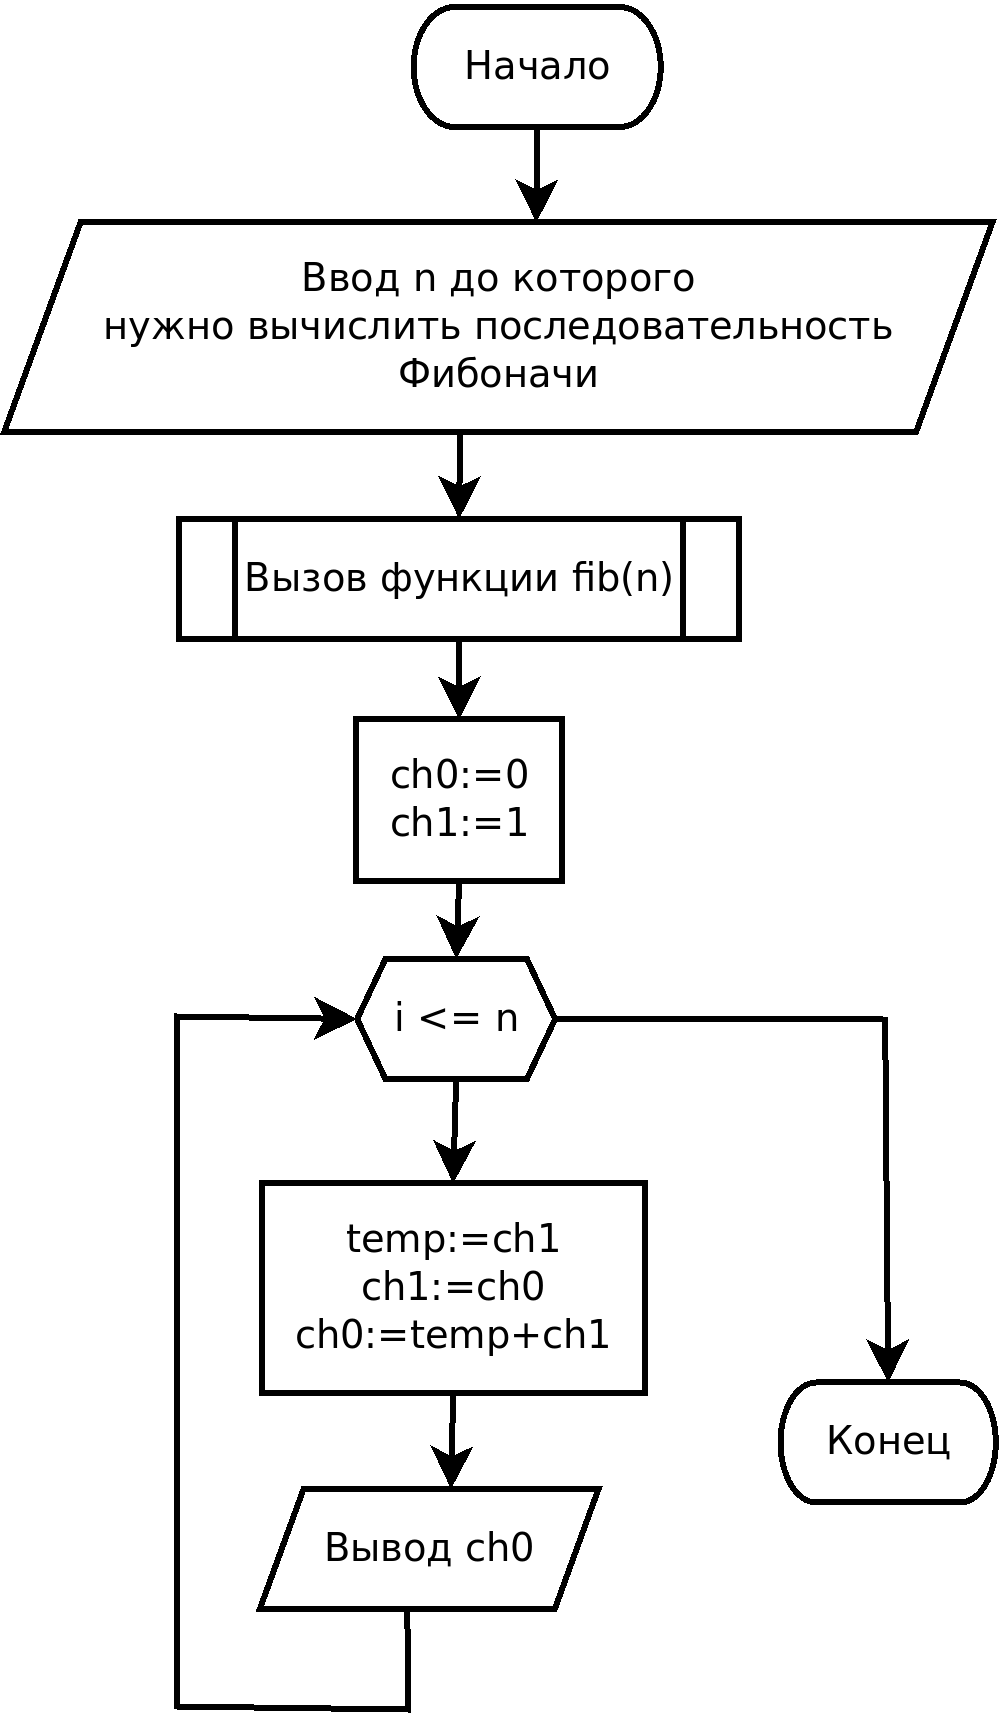
\includegraphics[width=0.5\textwidth]{./images/fibonacci.png}
    \caption{\centering\label{fig:example01}Пример рисунка в формате PNG.}
\end{figure}

Пример ссылки на рисунок в документе~\ref{fig:example02}.
\begin{figure}[h]
    \centering
    \includesvg[width=0.5\textwidth]{./images/fibonacci.svg}
    \caption{\centering\label{fig:example02}Пример рисунка в формате SVG.}
\end{figure}

Пример ссылки на таблицу в документе~\ref{tab:example01}.
\begin{table}[H]
\caption{\centering\label{tab:example01}Системные требования}
\begin{tabular}{|p{3 cm}|p{3 cm}|p{3 cm}|p{5 cm}|}
\hline
Минимальные требования & 1 & 2 & 3 \\ \hline
Версия операционной системы & 1 & 2 & 3 \\ \hline
Процессор & 1 & 2 & 3 \\ \hline
Графический API & 1 & 2 & 3 \\ \hline
\end{tabular}
\end{table}

Пример ссылки на таблицу в документе~\ref{tab:example02}.
\begin{table}[H]
\caption{\centering\label{tab:example02}Системные требования}
\begin{tabular}{|p{3 cm}|p{3 cm}|p{3 cm}|p{5 cm}|}
\hline
Минимальные требования & 1 & 2 & 3 \\ \hline
Версия операционной системы & 1 & 2 & 3 \\ \hline
Процессор & 1 & 2 & 3 \\ \hline
Графический API & 1 & 2 & 3 \\ \hline
\end{tabular}
\end{table}

Пример использования minted для оформления кода и ссылка на этот код~\ref{code:fibonacci}.
\begin{code}
\captionof{listing}{\centering\label{code:fibonacci}Пример программы вычисления n-ой последовательности Фибоначчи}
\vspace{-\baselineskip}\inputminted{python}{src/fibonacci.py}
\end{code}

Пример использования minted для оформления кода и ссылка на этот код~\ref{code:example02}.
\begin{code}
\captionof{listing}{\centering\label{code:example02}Сложение двух массивов параллельно десятью потоками (пример из https://ru.wikipedia.org/wiki/OpenMP)}
\vspace{-\baselineskip}\begin{minted}{C}
#include <stdio.h>
#include <omp.h>
#define N 100

int main(int argc, char *argv[]) {
  double a[N], b[N], c[N];
  int i;
  omp_set_dynamic(0); // запретить библиотеке openmp менять число потоков во время исполнения
  omp_set_num_threads(10); // установить число потоков в 10
  // инициализируем массивы
  for (i = 0; i < N; i++) {
      a[i] = i * 1.0;
      b[i] = i * 2.0;
  }
  // вычисляем сумму массивов
#pragma omp parallel for shared(a, b, c) private(i)
   for (i = 0; i < N; i++)
     c[i] = a[i] + b[i];

  printf ("%f\n", c[10]);
  return 0;
}
\end{minted}
\end{code}
